\begin{figure}[hb]
  \centering
  \begin{subfigure}[b]{.22\textwidth}
    \centering
    \begin{tikzpicture}
      \Vertices{figs/chapter2/mtt/mtt-vertices-sem.csv}
      \Edges{figs/chapter2/mtt/mtt-edges-sem.csv}
    \end{tikzpicture}
    \caption{SemR}
  \end{subfigure}
  \begin{subfigure}[b]{.22\textwidth}
    \centering
    \begin{tikzpicture}
      \Vertices{figs/chapter2/mtt/mtt-vertices-syn.csv}
      \Edges{figs/chapter2/mtt/mtt-edges-syn.csv}
    \end{tikzpicture}
    \caption{SyntR}
  \end{subfigure}
  \begin{subfigure}[b]{.22\textwidth}
    \centering
    \begin{tikzpicture}
      \Vertices{figs/chapter2/mtt/mtt-vertices-morph.csv}
      \Edges{figs/chapter2/mtt/mtt-edges-morph.csv}
    \end{tikzpicture}
    \caption{MorphR}
  \end{subfigure}
  \begin{subfigure}[b]{.22\textwidth}
    \centering
    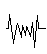
\includegraphics{figs/chapter2/mtt/wave.png}
    \caption{PhonR}
  \end{subfigure}
  \caption{語義-文字理論。}
  \label{fig:mtt}
\end{figure}